\section[Theorie]{Theorie \textnormal{\cite{pumpen}}}
\label{sec:theorie}

\subsection{Atomare Drehimpulse}

\begin{figure}[H]
	\centering
	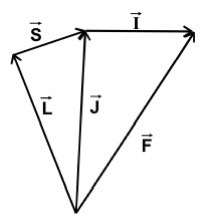
\includegraphics[width=0.25\linewidth]{content/grafik/drehimpulse.jpg}
	\caption{\cite{pumpen}}
	\label{fig:drehimpulse}
\end{figure}

\subsubsection{Hülle}

\begin{figure}[H]
	\centering
	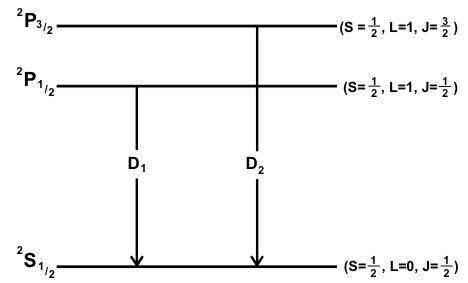
\includegraphics[width=0.5\linewidth]{content/grafik/duplett.jpg}
	\caption{\cite{pumpen}}
	\label{fig:duplett}
\end{figure}

\begin{figure}[H]
	\centering
	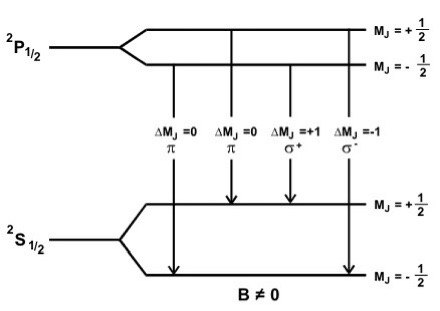
\includegraphics[width=0.55\linewidth]{content/grafik/zeeman.jpg}
	\caption{\cite{pumpen}}
	\label{fig:zeeman}
\end{figure}

\subsubsection{Kern}

\begin{figure}[H]
	\centering
	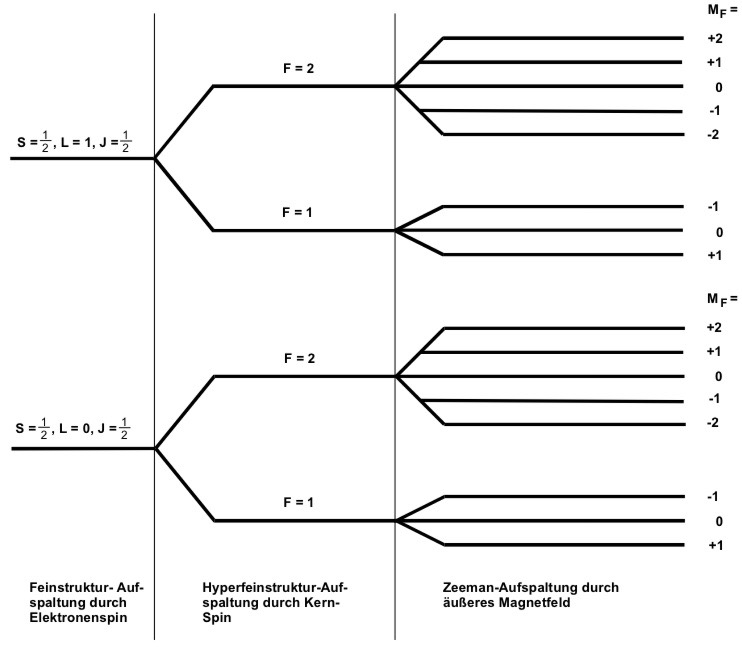
\includegraphics[width=0.7\linewidth]{content/grafik/hyperfein.jpg}
	\caption{\cite{pumpen}}
	\label{fig:hyperfein}
\end{figure}

\subsection{Optisches Pumpen}

\begin{figure}[H]
	\centering
	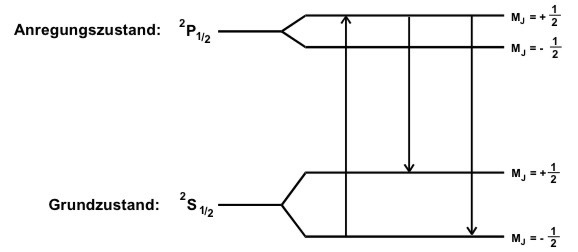
\includegraphics[width=0.65\linewidth]{content/grafik/pumpen.jpg}
	\caption{\cite{pumpen}}
	\label{fig:pumpen}
\end{figure}

\begin{figure}[H]
	\centering
	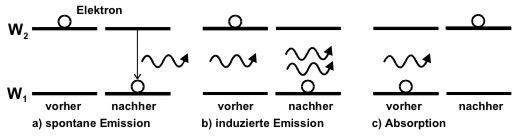
\includegraphics[width=0.75\linewidth]{content/grafik/uebergang.jpg}
	\caption{\cite{pumpen}}
	\label{fig:uebergang}
\end{figure}

\begin{figure}[H]
	\centering
	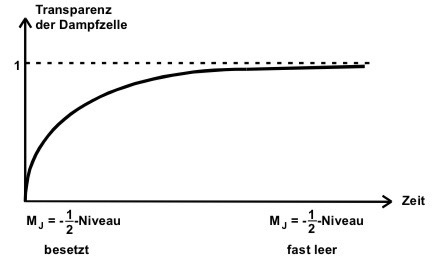
\includegraphics[width=0.6\linewidth]{content/grafik/transparenz.jpg}
	\caption{\cite{pumpen}}
	\label{fig:transparenz}
\end{figure}

\begin{figure}[H]
	\centering
	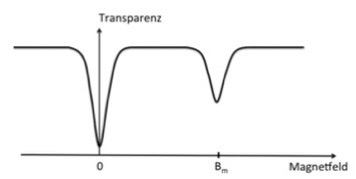
\includegraphics[width=0.6\linewidth]{content/grafik/minima.jpg}
	\caption{\cite{pumpen}}
	\label{fig:minima}
\end{figure}

\subsection{Zeeman Aufspaltung}

\subsection{Transiente Effekte}

\begin{figure}[H]
	\centering
	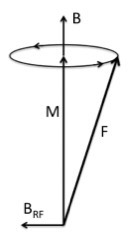
\includegraphics[width=0.2\linewidth]{content/grafik/praezession.jpg}
	\caption{\cite{pumpen}}
	\label{fig:praezession}
\end{figure}

